\documentclass[12pt]{article}

\usepackage{graphicx}
\usepackage[margin=1.0in]{geometry}
\usepackage{amsmath}
\usepackage{cases}
\usepackage{amsfonts}
\usepackage{amssymb}
\usepackage{grffile}
\usepackage{setspace}

\setlength\parindent{0pt}

\author{Xiaohui Chen \\EID: xc2388}
\title{M 362K Post-Class Homework 5}


\begin{document}
\maketitle
\begin{spacing}{1.9}

\section*{2-57}

\begin{figure}
  \centering
  % Requires \usepackage{graphicx}
  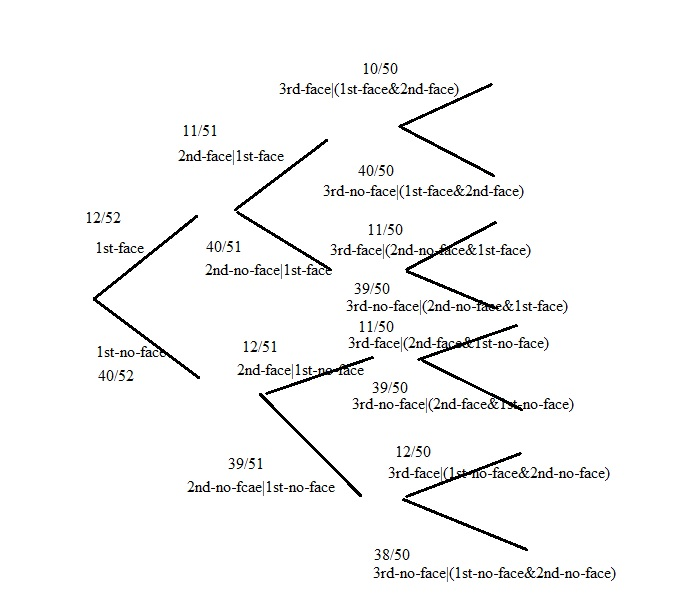
\includegraphics[width=6.5in]{out1}\\
  \caption{Tree diagram in 2-57}\label{out1}
\end{figure}

The tree diagram is shown in Figure \ref{out1} 

\subsection*{(a)}
$Pr(three\ faces)=\frac{10}{50}* \frac{11}{51}* \frac{12}{52}= \frac{11}{1105}$

\subsection*{(b)}
$Pr(at\ least\ two\ faces)=Pr(three\ faces)+Pr(two\ faces)= \frac{11}{1105}+\frac{12}{52}* \frac{11}{51}* \frac{40}{50} + \frac{12}{52}*\frac{40}{51}* \frac{11}{50}+ \frac{40}{52}* \frac{12}{51}*\frac{11}{50}=\frac{11}{85}$

\subsection*{(c)}
$Pr(3rd-face|(1st-face \cap 2nd-face))= \frac{10}{50}= \frac{1}{5}$

\subsection*{(d)}
$Pr(three\ faces|at\ least\ two\ faces)=\frac{Pr(three\ faces)}{Pr(at\ least\ two\ faces)}= \frac{\frac{11}{1105}}{\frac{11}{85}} = \frac{1}{13}$

\subsection*{(e)}
$Pr(at\ least\ two\ faces\cap Pr(last\ face))= \frac{10}{50}* \frac{11}{51}* \frac{12}{52} + \frac{11}{50}* \frac{40}{51}* \frac{12}{52}+ \frac{11}{50}* \frac{12}{51}* \frac{40}{52}= \frac{99}{1105}$

\section*{2-62}
From the question, we know that $Pr(heavy)=0.2$, $Pr(light)=0.3$ and $Pr(non)=0.5$

Let $Pr(die|non)=x$, then $Pr(die|light)=2x$ and $Pr(die|heavy)=4x$

$\therefore Pr(heavy|die)=\frac{Pr(die|heavy)*Pr(heavy)}{ Pr(die|heavy)*Pr(heavy)+ Pr(die|light)*Pr(light) + Pr(die|non)*Pr(non)}= \frac{4x*0.2}{4x*0.2 + 2x*0.3+ x*0.5} \approx 0.42$

Therefore the answer is (D)

\section*{2-63}
$Pr(16-20|accident)= $

$\frac{Pr(accident|16-20)*Pr(16-20)}{ Pr(accident|16-20)*Pr(16-20)+ Pr(accident|21-30)*Pr(21-30)+ Pr(accident|31-65)*Pr(31-65)+ Pr(accident|66-99)*Pr(66-99)}= \frac{0.06*0.08}{0.06*0.08+ 0.03*0.15+ 0.02*0.49+ 0.04*0.28} \approx 0.16$

Therefore the answer is (B)

\section*{Sample Exam 26}
$Pr(seven\ claims)=Pr(1st-0)*Pr(2nd-7)+ Pr(1st-1)*Pr(2nd-6)+ Pr(1st-2)*Pr(2nd-5)+ Pr(1st-3)*Pr(2nd-4)+ Pr(1st-4)*Pr(2nd-3)+ Pr(1st-5)*Pr(2nd-2)+ Pr(1st-6)*Pr(2nd-1)+ Pr(1st-7)*Pr(2nd-0)= \frac{1}{2}*\frac{1}{2^8} + \frac{1}{2^2}*\frac{1}{2^7}+ \frac{1}{2^3}*\frac{1}{2^6}+ \frac{1}{2^4}*\frac{1}{2^5}+ \frac{1}{2^5}*\frac{1}{2^4}+ \frac{1}{2^6}*\frac{1}{2^3}+ \frac{1}{2^7}*\frac{1}{2^2}+ \frac{1}{2^8}*\frac{1}{2^1}= \frac{1}{64}$

Therefore the answer is (D)

\end{spacing}
\end{document}